

\subsection{Ladder-Lottery Realization}

In their paper \textbf{Ladder-Lottery Realization} the authors provide 
a rather interesting puzzle in regards to ladder lotteries. The puzzle 
is known as the ladder-lottery realization problem. In order to understand
the problem, one must know what a \emph{multi-set} is. A \emph{multi-set}
is a set in which an element appears more than once. The exponent 
above the element indicates the number of times it appears in the set.
For example, given the following multi-set, $\{3^{2}, 2^{4}, 5^{1}\}$ 
the element $3$ appears twice in the set, the element $2$ appears four times
in the set and the element $5$ appears once in the set.
The ladder-lottery realization puzzle asks, given an arbitrary starting permutation 
and a multi-set of bars, 
is there a \emph{non-optimal} ladder lottery for the arbitrary permutation
that uses every bar in the multi-set the number 
of times it appears in the  multi-set. 
For an example of an affirmative solution to the ladder lottery realization problem, see figure --fig ref --.


\begin{figure}[!htp]
    \begin{center}
        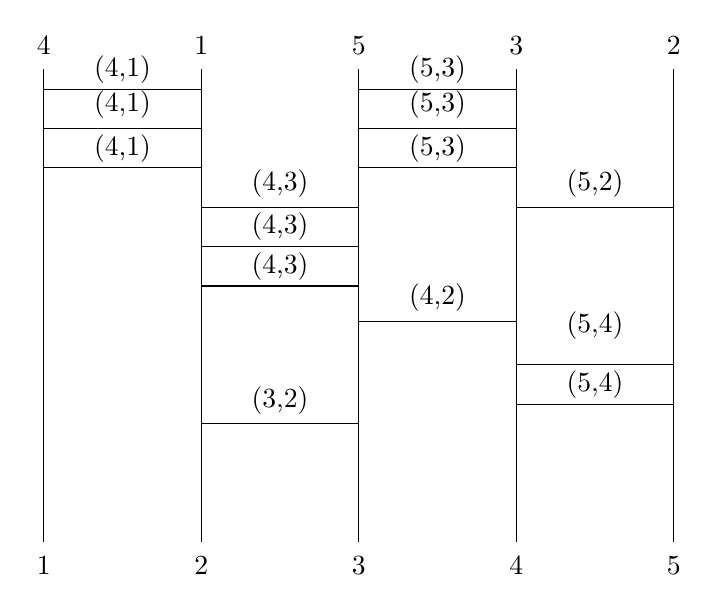
\begin{tikzpicture}
            \draw (0, 0) to (0, 6);
                \node at(0, -0.3){1};
                \node at(0, 6.3){4};
            \draw(2, 0) to (2, 6);
                \node at(2, -0.3){2};
                \node at(2, 6.3){1};
            \draw(4, 0) to (4, 6);
                \node at(4, 6.3){5};
                \node at(4, -0.3){3};
            \draw(6, 0) to (6, 6);
                \node at(6, 6.3){3};
                \node at(6, -0.3){4};
            \draw(8, 0) to (8, 6);
                \node at(8, 6.3){2};
                \node at(8, -0.3){5};

            %%draw the bars
                \node at(1, 6){(4,1)};
                    \draw(0, 5.75) to (2, 5.75);
            \draw(0, 5.25) to (2, 5.25);
                \node at(1, 5.55){(4,1)};
            \draw(0, 4.75) to (2, 4.75);
                \node at(1, 5){(4,1)};

            \draw(4, 5.75) to (6, 5.75);
                \node at(5, 6){(5,3)};
            \draw(4, 5.25) to (6, 5.25);
                \node at(5, 5.55){(5,3)};
            \draw(4, 4.75) to (6, 4.75);
                \node at(5, 5){(5,3)};

            \draw(2, 4.25) to (4, 4.25);
                \node at (3, 4.55){(4,3)};
            \draw(2, 3.75) to (4, 3.75);
                \node at (3, 4){(4,3)};
            \draw(2, 3.25) to (4, 3.25);
                \node at (3, 3.5){(4,3)};
            
            \draw(2, 1.5) to (4, 1.5);
                \node at(3, 1.8){(3,2)};
            
            \draw(4, 2.8) to (6, 2.8);
                \node at (5, 3.1){(4,2)};
            \draw(6, 4.25) to (8, 4.25);
                \node at (7, 4.55){(5,2)};
            
            \draw(6, 2.25) to (8, 2.25);
                \node at (7,2.75){(5,4)};
            
            \draw(6, 1.75) to (8, 1.75);
                \node at (7, 2){(5,4)};
            
        \end{tikzpicture}
    \end{center}
      


    \caption{An affirmative solution to the Ladder Lottery Realization Problem given a starting perumtation $(4,1,5,3,2)$ and the multi set of bars $\{(4,1)^{3}, (4,3)^{3}, (4,2)^{1}, (5,4)^{2}, (5,3)^{3}, (5,2)^{1},(3,2)^{1}\}$}
\end{figure}
\pagebreak
The authors prove that the ladder-lottery realization problem in NP-Hard
by reducing the ladder-lottery realization to the One-In-Three 3SAT, 
which has already been proven to be NP-Hard. The One-In-Three 3SAT 
problem is a problem such that given a set of variables $(X)$, a collection 
of \emph{disjuntcive clauses} $(C)$ which are disjunctive expressions of over 
literals of $X$. Each clause in $C$ contains exactly 
must contain three literals then is there a truth assignment for $X$ such that 
each clause in $C$ has exactly one true literal. For eaxmple, let 
$X=\{p, q, r, s, t\}$ and let $C=\{C_{p,q,s}, C_{r,q,s} C_{p,s,t}, C_{r,t,q}\}$,
the question is whether it is possible for each clause to have exactly one
true literal. The answer in this case is yes. If $p=T$, $r=T$, $q=F$, $s=F$
 and $t=T$ then all the clauses in $C$ have exactly one true literal. 
 The authors reduce the ladder lottery-realization problem to the
One-In-Three 3SAT problem by devising four gadgets. The result of 
the reduction is that the arbitrary starting permutation is equivelent 
to a derivation of the intial set of variables, $X$, in the One-In-Three 3SAT 
problem and the multi-set of bars is equivelent to a 
derivation of the intial set of clauses, $C$, in the One-In-Three 
3SAT problem.\par 
The authors note that there are two cases in which the ladder-lottery
realization problem can be solved in polynomial time. These cases 
include the follwing. First, if every bar in the multi-set appears
exactly once and every bar corresponds to a permutation, 
then an affirmative solution to the ladder-lottery realization 
instance can be demonstrated in polynomial time. 
Second, if there is an inversion in the perumutation and its bar appears in the multi-set an even 
number of times, then a negative solution to
the ladder-lottery realization instance
can be solved in polynomial time.\par